\section[Měření neutronů aktivační metodou]{Stanovení neutronových polí, účinných průřezů a štěpných výtěžků využitím aktivační techniky}

Většina důležitých informací je v otázkách 9-11.

\subsection{Aktivační měření s dozimetrickými foliemi}

Měření probíhá tak, že vložíme aktivační detektor (folie o známé tloušťce, hmotnosti a materiálu) do neutronového pole a poté za pomoci spektrometrie určíme reakční rychlost:

\begin{equation}
    \boxed{R = \int_{E_{min}}^{E_{max}} \phi(E) \sigma(E) \: \text{d}E = \dfrac{S \lambda \dfrac{t_\text{real}}{t_\text{live}}}{N_0 \: \varepsilon \: I \: (1-e^{-\lambda t_a}) \: e^{-\lambda t_v} \: (1-e^{-\lambda t_\text{real}}),}}
\end{equation}

případně produkční rychlost (furt ty samé vztahy):

\begin{equation}
    \boxed{P =  \dfrac{S \lambda \dfrac{t_\text{real}}{t_\text{live}}}{\varepsilon \: I \: (1-e^{-\lambda t_a}) \: e^{-\lambda t_v} \: (1-e^{-\lambda t_\text{real}}).}}
\end{equation}

Tato měření pak pomohou pomoct v dalších odvětvích (teď mimo NAA, té se věnuje předešlá otázka).

\subsubsection{Měření účinných průřezů}

Hojně využívané pro měření účinných průřezů prahových reakcí (na urychlovači). Jako zdroj neutonů se použije svazek protonů, které odstřelují tenkou Li folii (p + Li), což produkuje proud kvazimonoenergetických neutronů, které jsou dobře odlišitelné od pozadí. Dále možné využít beryliový terčík (p + Be).

\begin{figure}[H]
    \centering
    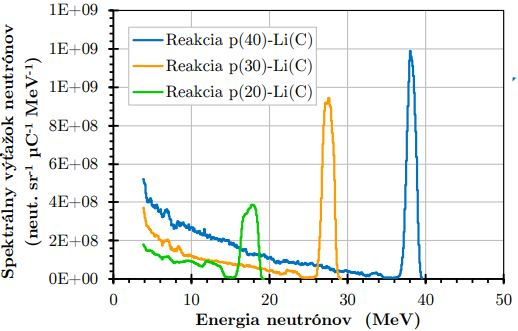
\includegraphics[width=0.5\textwidth]{img/p+Li_E.JPG}
    \caption{Neutronové spektrum pro reakci (p + Li).}
\end{figure}

Tím, jak měním rychlost primárních protonů jsem schopný sekundární neutronový peak posouvat do různých energiích. Tyto sekundární neutrony poté ozařují zkoumaný materiál, jehož účinný průřez měřím. Takto změřím někoik bodů (dle energie), které poté vyhodnocuji a dle čehož stanovím závislost $\sigma$ na $E$. Tato metoda se využívá v ÚJF AV ČR v Řeži.

\subsubsection{Spektrometrie neutronových polí}

Spektrometrii neutronů je věnována celá předchozí otázka, tahle kapitolka je pouze o smektrometrii aktivační technikou. Ve zkoumaném neutronovém poli se ozáří několik odlišných aktivačních detektorů: Cd, Mo, Y, Cu, In, Co apod., přičemž materiály se vybírají podle toho, jak jsou citlivé v jiných oblastech energie neutronů.

Po ozáření opět proběhne gamma spektrometrie a u každé folie se stanoví sada reakčních rychlostí. Jelikož známe průběhy účinných průřezů na těchto materiálech, je pak možné zpětně zrekonstruovat neutronové spektrum. K tomu se využívají různé kódy, my pracovali s kódem SAND-II (podobně jako v případě měření Bonnerovými sférami).

\begin{figure}[H]
    \centering
    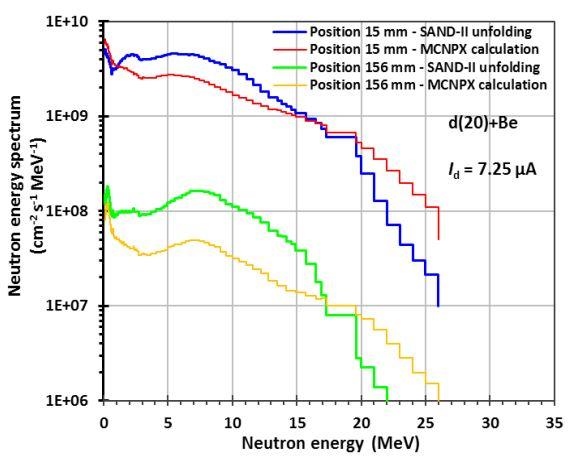
\includegraphics[width=0.5\textwidth]{img/spektrum_aktivacne.JPG}
    \caption{Zpětná rekompozice neutronového spektra pro reakci (d + Be).}
\end{figure}

\subsubsection{Stanovení štěpných výtěžků}


Aktivační metoda (neutron activation analysis, NAA) představuje klíčový nástroj pro kvantitativní analýzu štěpných produktů vznikajících při štěpení těžkých jader, jako je $^{235}$U nebo $^{239}$Pu. Tato metoda využívá měření gama záření emitovaného radionuklidy po jejich aktivaci neutrony a umožňuje stanovit relativní štěpné výtěžky jednotlivých produktů s vysokou přesností. Tato práce se zaměřuje na detailní popis principů NAA, její aplikaci na výpočet štěpných výtěžků a diskusi výhod a omezení této metody.

Štěpné výtěžky představují základní charakteristiku jaderného štěpení, vyjadřující relativní množství jednotlivých produktů vznikajících při této reakci. Přesné stanovení těchto výtěžků je nezbytné pro mnoho aplikací, včetně návrhu jaderných reaktorů, správy jaderného odpadu a základního výzkumu jaderné fyziky. Aktivační metoda (NAA) nabízí možnost měření s vysokou citlivostí a selektivitou, což ji činí oblíbenou pro analýzu produktů štěpení.

\subsubsection*{Princip metody}

NAA je analytická technika založená na ozařování vzorku neutrony a následném měření gama záření emitovaného radionuklidy. Celý proces lze rozdělit do následujících kroků:

\begin{enumerate}
    \item Vzorek obsahující štěpný materiál (např. $^{235}$U nebo $^{239}$Pu) je umístěn do vhodného kontejneru, který odolá neutronovému ozařování. Velikost a geometrie vzorku jsou optimalizovány pro dosažení rovnoměrného ozáření.
    \item Vzorek je ozářen neutrony ve zdroji, například v jaderném reaktoru. Během ozáření probíhá štěpení těžkých jader, přičemž vznikají produkty štěpení, které jsou často samy o sobě radioaktivní. Současně dochází k aktivaci přítomných prvků.
    \item Po ozařování je vzorek přemístěn do gama spektrometru. Radioaktivní produkty emitují gama záření, jehož energie jsou charakteristické pro konkrétní radionuklidy. Intenzita jednotlivých gama čar je přímo úměrná množství daného radionuklidu ve vzorku.
    \item Na základě změřených intenzit gama záření a znalosti detekční účinnosti, poločasů rozpadu a dalších parametrů lze vypočítat počet jader jednotlivých produktů štěpení. Relativní štěpné výtěžky se stanoví podle vztahu:
\begin{equation}
    \boxed{Y_i = \frac{N_i}{\sum_j N_j},}
\end{equation}
kde $N_i$ je počet jader i-tého produktu a $\sum_j N_j$ je celkový počet jader všech detekovaných produktů štěpení.
\end{enumerate}

\textbf{Výhody:}

\begin{itemize}
    \item Vysoká citlivost: Detekce stopových množství radionuklidů.
    \item Selektivita: Identifikace specifických radionuklidů díky charakteristickým energiím gama záření.
    \item Nedestruktivní charakter: Vzorek lze použít pro další analýzu.
\end{itemize}

\textbf{Omezení:}

\begin{itemize}
    \item Vyžaduje přístup k neutronovému zdroji, což omezuje její dostupnost.
    \item Náročné zpracování dat, zejména při překryvu gama čar.
    \item Manipulace s radioaktivními vzorky vyžaduje přísná bezpečnostní opatření.
\end{itemize}

\textbf{Aplikace:}

Metoda NAA je široce využívána v následujících oblastech:

\begin{itemize}
    \item Studium produktů štěpení při různých energiích neutronů.
    \item Výzkum vlastností jaderného paliva.
    \item Analýza radioaktivních odpadů.
\end{itemize}

Stanovení štěpných výtěžků pomocí aktivační metody je účinným nástrojem pro studium jaderných procesů. Tato metoda poskytuje přesná a spolehlivá data o relativních výtěžcích jednotlivých štěpných produktů, což přispívá k hlubšímu pochopení jaderného štěpení a jeho aplikací.
